\documentclass{beamer}

\usepackage{minted}
\usemintedstyle{eclipse}

\useoutertheme{infolines}
\setbeamertemplate{headline}{}
\setbeamertemplate{footline}{
  \hfill
  \usebeamercolor[fg]{page number in head/foot}
  \usebeamerfont{page number in head/foot}
  \insertpagenumber\kern1em\vskip10pt
}
\setbeamertemplate{navigation symbols}{}

\usepackage{tikz}
\usetikzlibrary{arrows}

\title{Lightweight Functional Logic Meta-Programming}
\subtitle{in Scala}
\author{Nada Amin, Tiark Rompf}
\institute{LAMP, EPFL}
\date{March 4, 2014}

\begin{document}

\frame{\titlepage}

\begin{frame}[fragile]{Logic Programming (Prolog)}
\begin{columns}
\begin{column}[t]{8cm}
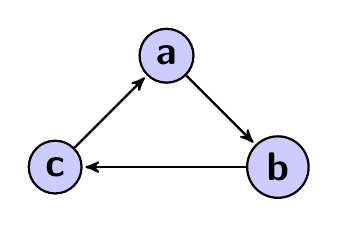
\begin{tikzpicture}[->,>=stealth',shorten >=1pt,auto,node distance=2cm,
  thick,main node/.style={circle,fill=blue!20,draw,font=\sffamily\Large\bfseries}]

  \node[main node] (1) {a};
  \node[main node] (2) [below right of=1] {b};
  \node[main node] (3) [below left of=1] {c};

  \path[every node/.style={font=\sffamily\small}]
    (1) edge node [right] {} (2)
    (2) edge node [right] {} (3)
    (3) edge node [right] {} (1);

\end{tikzpicture}
\begin{minted}{prolog}
edge(a,b).
edge(b,c).
edge(c,a).

path(X, Y) :- edge(X, Y).
path(X, Z) :- edge(X, Y), path(Y, Z).
\end{minted}
\end{column}
\begin{column}[t]{4cm}
\begin{minted}{prolog}
?- edge(a, X).
X = b.

?- edge(X, a).
X = c.

?- path(a, X).
X = b ;
X = c ;
X = a ;
X = b .
\end{minted}
\end{column}
\end{columns}
\end{frame}

\begin{frame}[fragile]{Logic Programming (Scala)}
\begin{minted}{scala}
def edge(x: Exp[String], y: Exp[String]): Rel =
  (x === "a") && (y === "b") ||
  (x === "b") && (y === "c") ||
  (x === "c") && (y === "a")

def path[T](x: Exp[T], y: Exp[T]): Rel =
  edge(x,y) ||
  exists[T] { z => edge(x,z) && path(y,b) }

// Queries
run[(String,String)] { case Pair(x,y) => edge(x,y) }
//=> pair(a,b), pair(b,c), pair(c,a)

runN[String](10) { q => path("a",q) }
//=> b, c, a, b, c, a, b, c, a, b
\end{minted}
\end{frame}

\begin{frame}[fragile]{Deep Linguistic Reuse: OO Encapsulation}
\begin{minted}{scala}
trait Graph[T] {
  def edge(x: Exp[T], y: Exp[T]): Rel
  def path(x: Exp[T], y: Exp[T]): Rel =
    edge(x,y) ||
    exists[T] { z => edge(x,z) && path(y,b) }
}
val g = new Graph[String] {
  def edge(x:Exp[String],y:Exp[String]) =
    (x === "a") && (y === "b") ||
    (x === "b") && (y === "c") ||
    (x === "c") && (y === "a")
}
\end{minted}
\end{frame}

\begin{frame}[fragile]{Deep Linguistic Reuse: Type Classes}
\begin{minted}{scala}
trait Ord[T] { def lt(x:Exp[T],y:Exp[T]): Rel }

implicit class OrdOps[T:Ord](x:Exp[T]) {
  def <(y:Exp[T]): Rel =
    implicitly[Ord[T]].lt(x,y)
}

implicit val ordNat = new Ord[Int] {
  def lt(x:Exp[Int],y:Exp[Int]): Rel =
    // ... elided
}


run[Int] { q => q < 4 } //=> 0,1,2,3
\end{minted}
\end{frame}

\begin{frame}[fragile]{Type Classes: Lexicographic Ordering on Polymorphic Lists}
\begin{minted}{scala}
implicit def ordList[T:Ord] = new Ord[List[T]] {
  def lt(as:Exp[List[T]],bs:Exp[List[T]]): Rel = 
    exists[T,List[T]] { (b,bs1) => 
      (bs === cons(b,bs1)) && {
      (as === nil) || exists[T,List[T]] { (a,as1) =>
      (as === cons(a,as1)) && {
      (a < b) || (a === b) && (as1 < bs1) }}}}

run[List[Int]] { q => q < List(0,1,2) }
//=> nil
//   cons(z,nil)
//   cons(z,cons(z,x0))
//   cons(z,cons(s(z),nil)),
//   cons(z,cons(s(z),cons(z,x0)))
//   cons(z,cons(s(z),cons(s(z),x0)))
\end{minted}
\end{frame}

\begin{frame}[fragile]{Type Classes: Run Queries Forwards and Backwards}
\begin{minted}{scala}
run[String] { q =>
  val t = tree(List(1,1,1) -> "a",
               List(1,2,2) -> "b",
               List(2,1,1) -> "c")
  lookup(t,List(1,2,2),q)
} //=> b
run[Int] { q =>
  val t = tree(List(1,1,1) -> "a",
               cons(q,List(2,2)) -> "b",
               List(2,2,2) -> "c")
  lookup(t,List(1,2,2),"b")
} //=> 1
\end{minted}
\end{frame}

\begin{frame}[fragile]{Vanilla Meta-Interpreter (Prolog)}
\begin{minted}{prolog}
/*
  A meta-interpreter for pure Prolog (Art of Prolog, 17.5)

  solve(Goal) :-
     Goal is true given the pure Prolog program defined by
     clause/2.
*/

     solve(true).
     solve((A,B)) :- solve(A), solve(B).
     solve(A) :- clause(A,B), solve(B).
\end{minted}
\end{frame}

\begin{frame}[fragile]{Tracing Meta-Interpreter (Prolog)}
\begin{minted}{prolog}
/*  
  A tracer for Prolog (Art of Prolog 17.7)
*/
		 
solve_trace(Goal) :-
	solve_trace(Goal,0).
     solve_trace(true,Depth) :- !.
     solve_trace((A,B),Depth) :-  !,
        solve_trace(A,Depth), solve_trace(B,Depth). 
     solve_trace(A,Depth) :-  
	builtin(A), !, A, display(A,Depth), nl.
     solve_trace(A,Depth) :-
        clause(A,B), 
	display(A,Depth), nl,
	Depth1 is Depth + 1, 
	solve_trace(B,Depth1).
\end{minted}
\end{frame}

\begin{frame}[fragile]{Tracing (Scala)}
\begin{minted}{scala}
val globalTrace = DVar(nil: Exp[List[List[String]]])
def path(x: Exp[T], y: Exp[T]): Rel = {
  globalTrace := cons(term("path",List(x,y)), globalTrace())
  edge(x,y) || exists[T] { z => edge(x,z) && path(y,b) }
}
\end{minted}
\end{frame}

\begin{frame}[fragile]{Modular Tracing (Scala)}
\begin{minted}{scala}
trait TracingGraph[T] extends Graph[T] {
  override def path(x:Exp[T],y:Exp[T]) =
    rule("path")(super.path)(x,y)
}
// tracing logic
val globalTrace = DVar(nil: Exp[List[List[String]]])
def rule[T,U](s: String)(f: (Exp[T],Exp[U]) => Rel):
  (Exp[T],Exp[U]) => Rel =
  { (a,b) =>
    globalTrace := cons(term(s,List(a,b)), globalTrace())
    f(a,b)
  }

runN[(String,List[String])](5) { case Pair(q1,q2) =>
      g.path("a",q1) && globalTrace() === q2 }
//=> pair(b,cons(path(a,b),nil)),
//   pair(c,cons(path(b,c),cons(path(a,c),nil))), ...
\end{minted}
\end{frame}

\begin{frame}[fragile]{Probabilistic Logic Computation}
\begin{minted}{scala}
val theprob = DVar(1.0)
def flip(p: Double)(a: => Rel)(b: => Rel): Rel =
  { theprob := theprob() * p; a } ||
  { theprob := theprob() * (1.0 - p); b }

runN[(Boolean,Double)](3) { case Pair(c,p) =>
  flip(0.2,c) && { p === theprob() } }
//=> pair(true,0.2), pair(false,0.8)
\end{minted}
\end{frame}

\begin{frame}[fragile]{Clause Reification as Controlled Side Effect (Ex.)}
\begin{minted}{scala}
var allclauses = Map[String,Clause]()
def reifyClause(goal: => Rel)(
    head: Exp[Goal], body: Exp[List[Goal]]): Rel =
  reifyGoals(goal)(cons(head,nil)) &&
  allclauses(extractKey(head))(head,body)
run[List[Any]] { q =>
  exists[Goal,List[Goal]] { (head,body) =>
    q === cons("to prove", cons(head, 
          cons("prove", cons(body, nil)))) &&
    reifyClause(path(g)(fresh,fresh))(head,body)
  }
}
// cons(to prove,cons(path(a,b),cons(prove,cons(nil,nil)))),
// ... 2 more
// cons(to prove,cons(path(a,x0),
//   cons(prove,cons(cons(path(b,x0),nil),nil)))), 
// ... 2 more
\end{minted}
\end{frame}

\begin{frame}[fragile]{Clause Reification as Controlled Side Effect (Impl.)}
\begin{minted}{scala}
val moregoals = DVar(fresh[List[Goal]])
def reifyGoals(goal: => Rel)(goals: Exp[List[Goal]]): Rel = {
  moregoals := goals
  goal && moregoals() === nil
}
def reflectGoal(goal: Exp[Goal]): Rel = {
  val hole = moregoals()
  moregoals := fresh
  hole === cons(goal,moregoals())
}
// reifyGoals(reflectGoal("path(a,b)")
//=>  "cons(path(a,b),nil)"

def rule[A,B](s: String)(f:(Exp[A], Exp[B]) => Rel) = {
  // ...
}
\end{minted}
\end{frame}

\begin{frame}[fragile]{Tabling: Semantics of Memoization}
Excerpt from Memoing for Logic Programs by David S. Warren:
\tiny
Intuitively, we think of a machine that is carrying out a nondeterministic procedure as duplicating itself at a point of choice, and as disappearing when it encounters failure. Thus at any time, we have a set of deterministic machines computing away. The set gets larger when any one has to make a nondeterministic choice, and it gets smaller when any one fails. To add memoing, we imagine a single global table containing every procedure call that has been made by any machine, and for each such call, the answers that have been returned for it. Since the situation is nondeterministic, there may be none, one, or many answers for any single call. Now each machine, before it makes a procedure call, looks in the global table to see if the call has already been made. If not, it adds the call to the table and continues computing. During its computation, whenever a machine returns from a procedure, it finds the associated call in the global table, adds the answer it has just computed, and continues computing. (If the answer is already in the table, then this answer is a duplicate, and the machine fails.) When a procedure is about to be called, if the call is found to be already in the table, then for each associated answer in the table, the machine must fork off a new copy of itself to continue the computation with that answer. It is possible that not all the answers are in the table at this time; some may still be in the process of being computed by other machines and will show up later. Thus when a machine encounters a call already in the table, it forks off copies of itself to continue with the answers that are there, and it remains suspended on that table entry. Then whenever a new answer gets added to the table, the suspended machine makes a duplicate of itself to continue computing with that new answer. When a machine finishes its computation successfully, it disappears. The entire computation is complete when (and if) no machines are computing.
\end{frame}

\begin{frame}[fragile]{Conclusion}
\begin{itemize}
\item like in Lightweight Modular Staging
\begin{itemize}
\item exploit deep linguistic reuse
\item use virtualization instead of reflection for meta-programming
\end{itemize}
\item further reading
\begin{itemize}
\item dynamic variables local to search thread\\
{\tiny\url{http://okmij.org/ftp/Computation/dynamic-binding.html}}
\item tutorial on purely embedding logic programming in functional host\\
accessible to undergraduate students\\
{\tiny\url{http://webyrd.net/scheme-2013/papers/HemannMuKanren2013.pdf}}
\end{itemize}
\end{itemize}
\end{frame}

\begin{frame}[fragile]{The Future: Embedding Logical Frameworks in Scala}
\begin{itemize}
\item Possible improvements over Twelf
\begin{itemize}
\item custom search strategies
\item meta-level abstraction: e.g. parametric lists
\item do better than copy'n'paste modularity
\item notion of functions: once you proved a relation is a function, use it as a function
\item z3 for totality / coverage checking
\item z3 as logic/constraint solving engine
\end{itemize}
\end{itemize}
\end{frame}

\end{document}
